\documentclass[10pt]{article}
\usepackage[letterpaper,margin=0.725in]{geometry}

\usepackage{fancyhdr}
\usepackage{amsmath}
\usepackage{mathtools}
\usepackage{hyperref}
\usepackage[english]{babel}
\usepackage{graphicx}
\usepackage{float}
\usepackage{caption}
\usepackage{amssymb}
\usepackage{caption}
\usepackage{amstext} % for \text macro
\usepackage{array}   % for \newcolumntype macro
\allowdisplaybreaks

\usepackage[T1]{fontenc}
\usepackage[numbered,framed]{matlab-prettifier}

\hypersetup{ colorlinks=true, linkcolor=blue}

\DeclareMathOperator{\atantwo}{atan2}
\newcolumntype{C}{>{$}c<{$}} % math-mode version of "l" column type

\pagestyle{fancy}
\lhead{RBE 500 - PA \#2 \newline Team 2: Peter Campellone, Aislin Hanscom, Christopher Poole}
\rhead{Due: 7/13/2021}

\begin{document}

\setlength{\abovedisplayskip}{6pt}
\setlength{\belowdisplayskip}{3pt}
\setlength{\abovedisplayshortskip}{4pt}
\setlength{\belowdisplayshortskip}{4pt}

\textbf{Package overview:}
\begin{itemize}
	\item Inside \texttt{catkin\_ws/src}, the main package is \texttt{scara\_robot}. It does not directly contain any nodes or launch files, but is a way to organize all of the other nodes.
	\begin{itemize}
		\item New package:
		\begin{itemize}
			\item The \texttt{pd\_controller} package implements a proportional and derivative controller for joint 3 (prismatic joint). The controller functions by reading the current joint position, calculating the necessary input into the joint, and applying the input force using the \texttt{gazebo/apply\_joint\_effort} topic.
		\end{itemize}
		
		\item Old packages (from PA \#1):
		\begin{itemize}
			\item The \texttt{scara\_gazebo} package includes the launch files for the gazebo world.
			\item The \texttt{scara\_description} package includes the URDF files for the robot as well as the rviz launch files.
			\item The \texttt{gazebo\_publish} package includes the launch file to allow for the joint states to be published from gazebo.
			\item The \texttt{scara\_forward\_kinematics} folder is the pub/sub package that subscribes to the joint states, calculates the forward kinematics, and publishes the pose.
			\item The \texttt{scara\_inverse\_kinematics} folder is the service/client package that ingests a desired end effector pose and returns the joint position.
		\end{itemize}
	\end{itemize}
\end{itemize}

\begin{enumerate}
	\item Fix all of the joints except the last joint by changing the joint type field of the corresponding joints to "fixed" in the robot description file.
	
	\item Write a position controller node.
	
	\begin{itemize}
		\item Get positions from Gazebo and be able to send joint efforts.
		
		\item Design PD controller (tune gains, don't calculate)
		
		\item Implement service that takes in a reference (desired) position for the last joint.
		
		\item Record both the reference position and current position in a text file. Plot the comparison in MATLAB.
		
	\end{itemize}

	We need to start by determining the E.O.M. of our third link for our controller:
	
	\begin{minipage}[h]{0.3\textwidth}
		\centering
		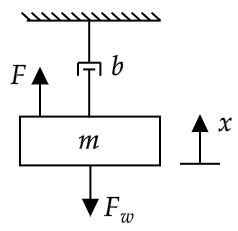
\includegraphics[width=0.7\textwidth]{figures/mass_damper.png}
	\end{minipage}
	\begin{minipage}[h]{0.5\textwidth}
		\begin{align*}
			&\sum{F} = m a \Rightarrow F - b \dot{x} - F_w = m \ddot{x} \\
			&m \ddot{x} + b \dot{x} + F_w = F \\
			&H(s) = \frac{X(s)}{F(s)} = \frac{1}{m s^2 + b s + F_w}
		\end{align*}
	\end{minipage}

	Steps to run:
	
	\begin{enumerate}
		\item \texttt{catkin\_make}
		\item \texttt{source devel/setup.bash}
		\item \texttt{roslaunch scara\_gazebo scara\_world.launch}
		
	\end{enumerate}

\end{enumerate}
\end{document}



